\documentclass[portrait,color=UCLmidgreen,margin=1.5cm,bannerheight=8cm,logoheight=3.5cm]{uclposter}
\usepackage{tikz}
\usepackage[scaled=1.2]{helvet}
\renewcommand\familydefault{\sfdefault} 
\usepackage[T1]{fontenc}
\usepackage[raster]{tcolorbox}
\usepackage{grid-system}

\title{Performance characterisation of 8-bit RISC and OISC architectures}

%\affil[1]{UCL Electronic And Electrical Engineering}

\begin{document}

%\tikz\node[opacity=0.3,inner sep=0]{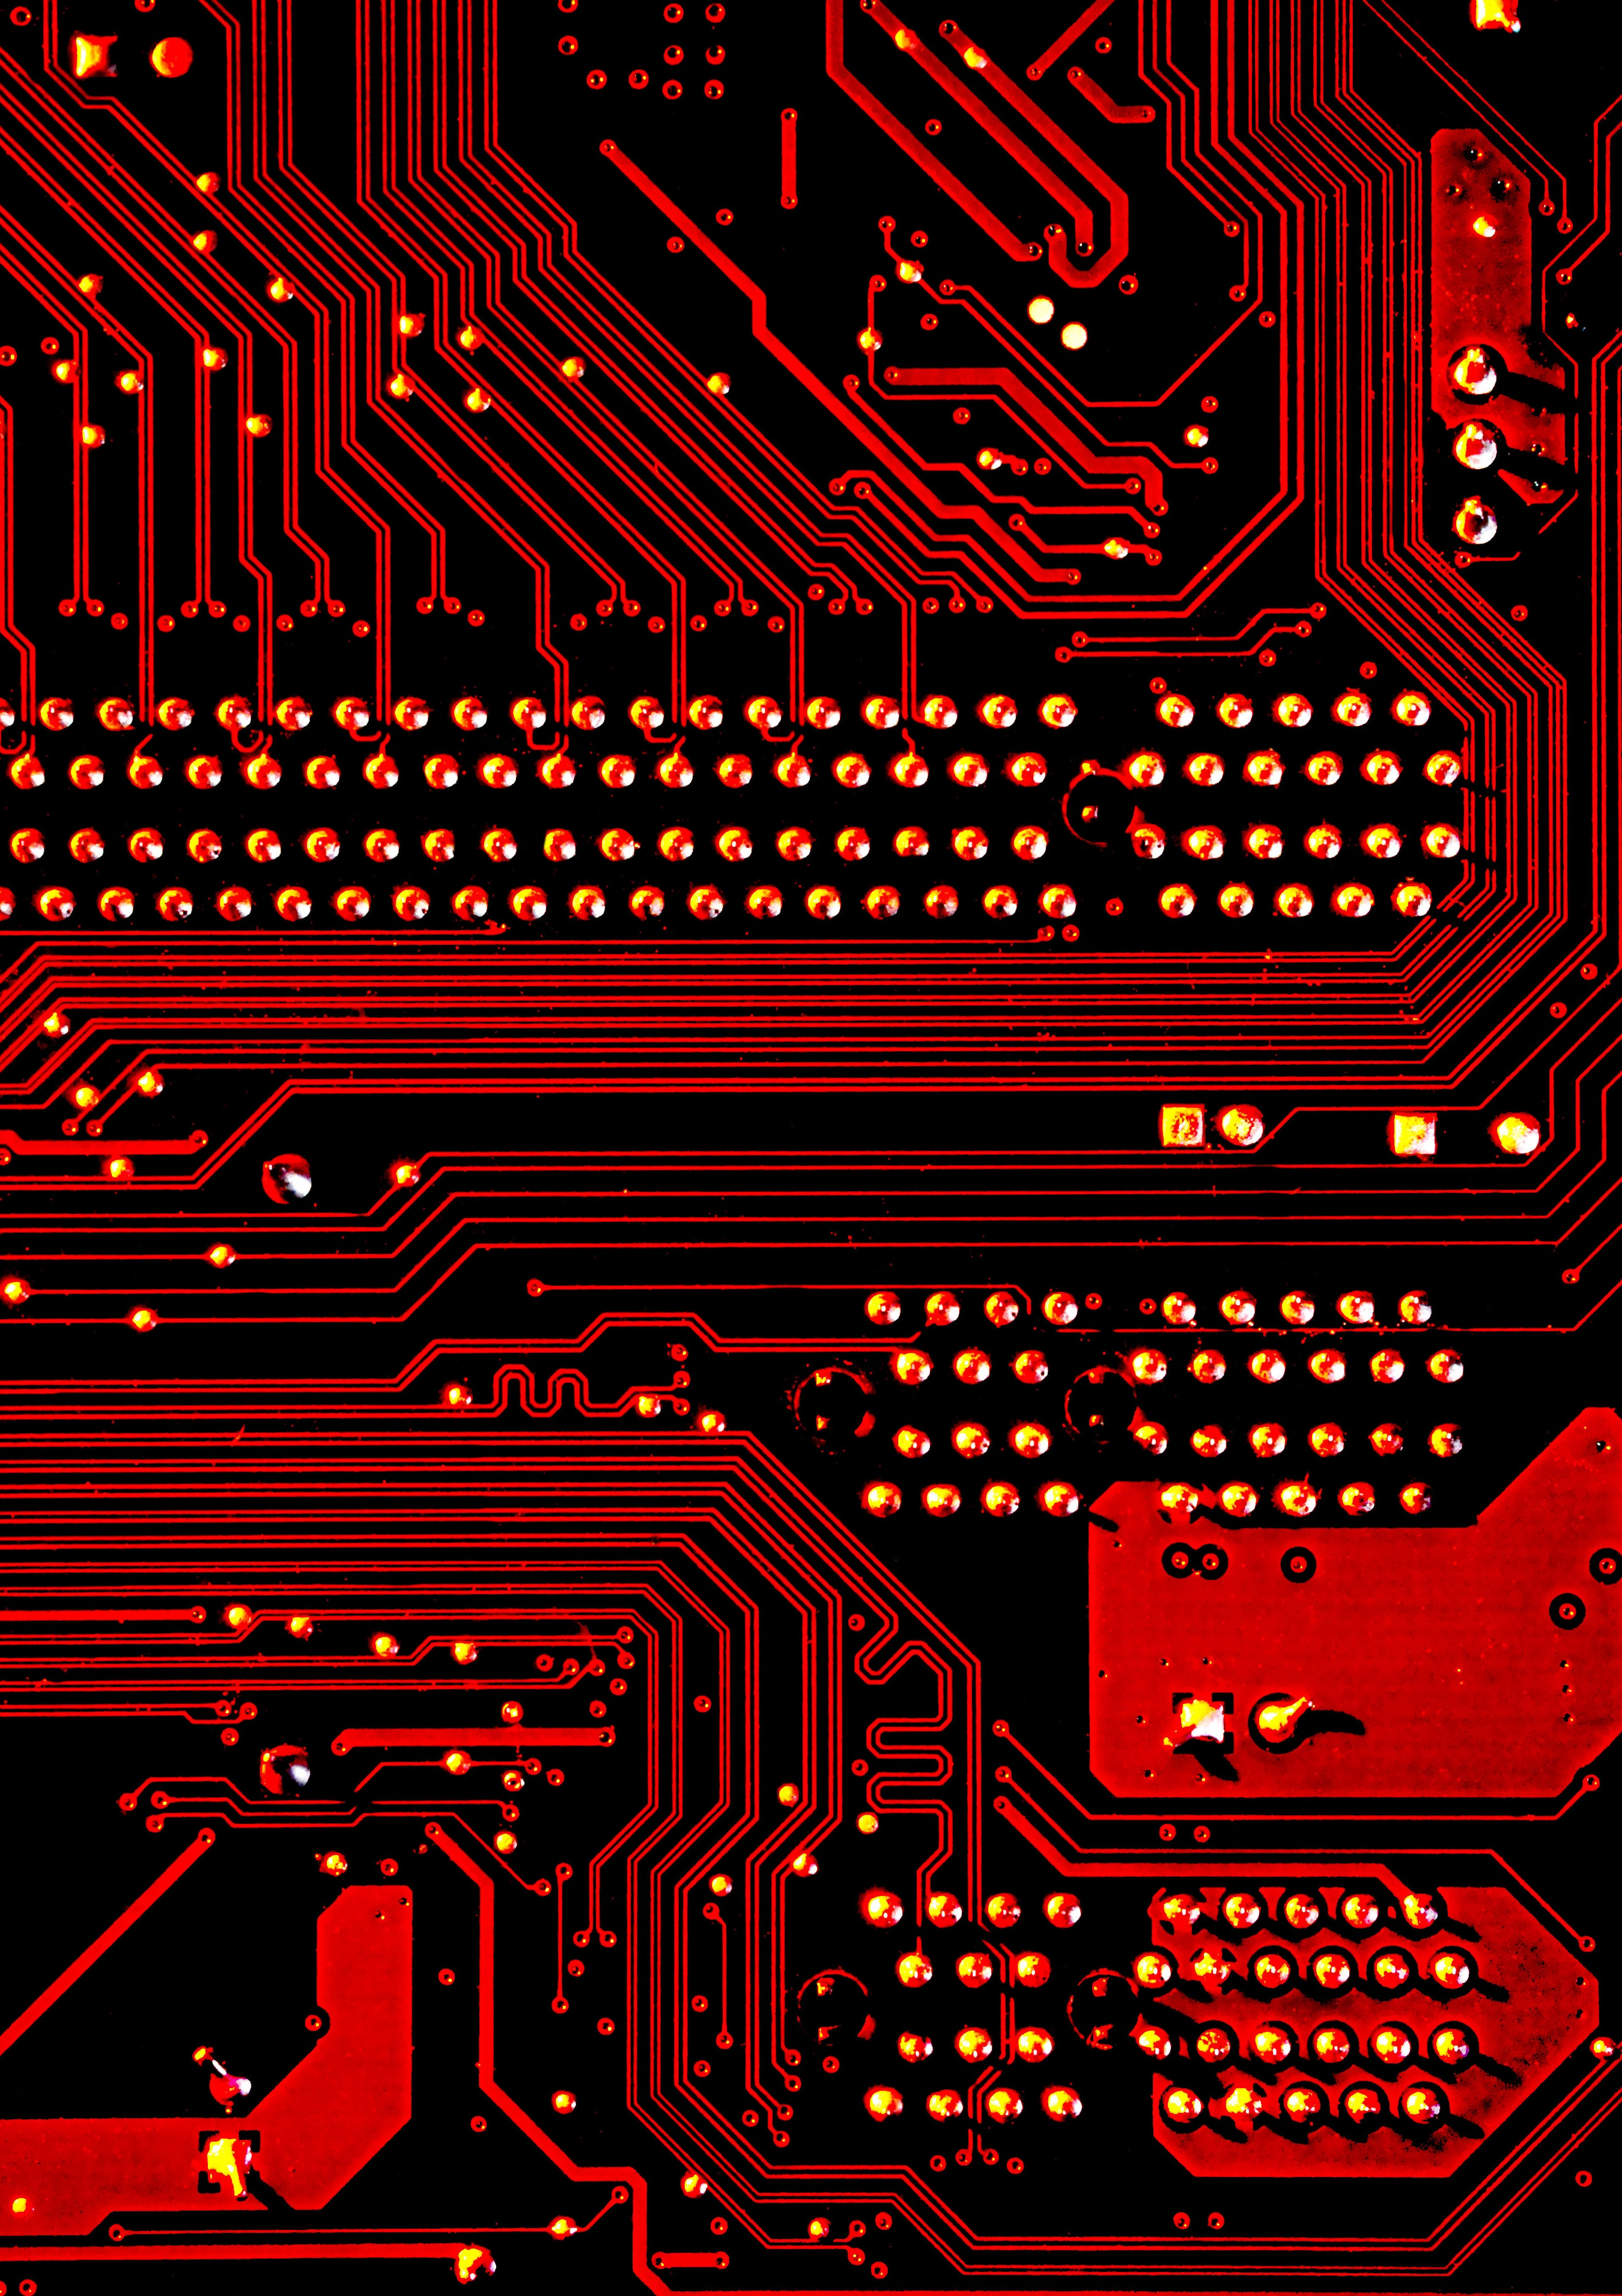
\includegraphics[height=\paperheight,width=\paperwidth]{background.jpg}}
%\tikz[remember picture,overlay] \node[opacity=0.3,outer sep=0pt] at (current page.center){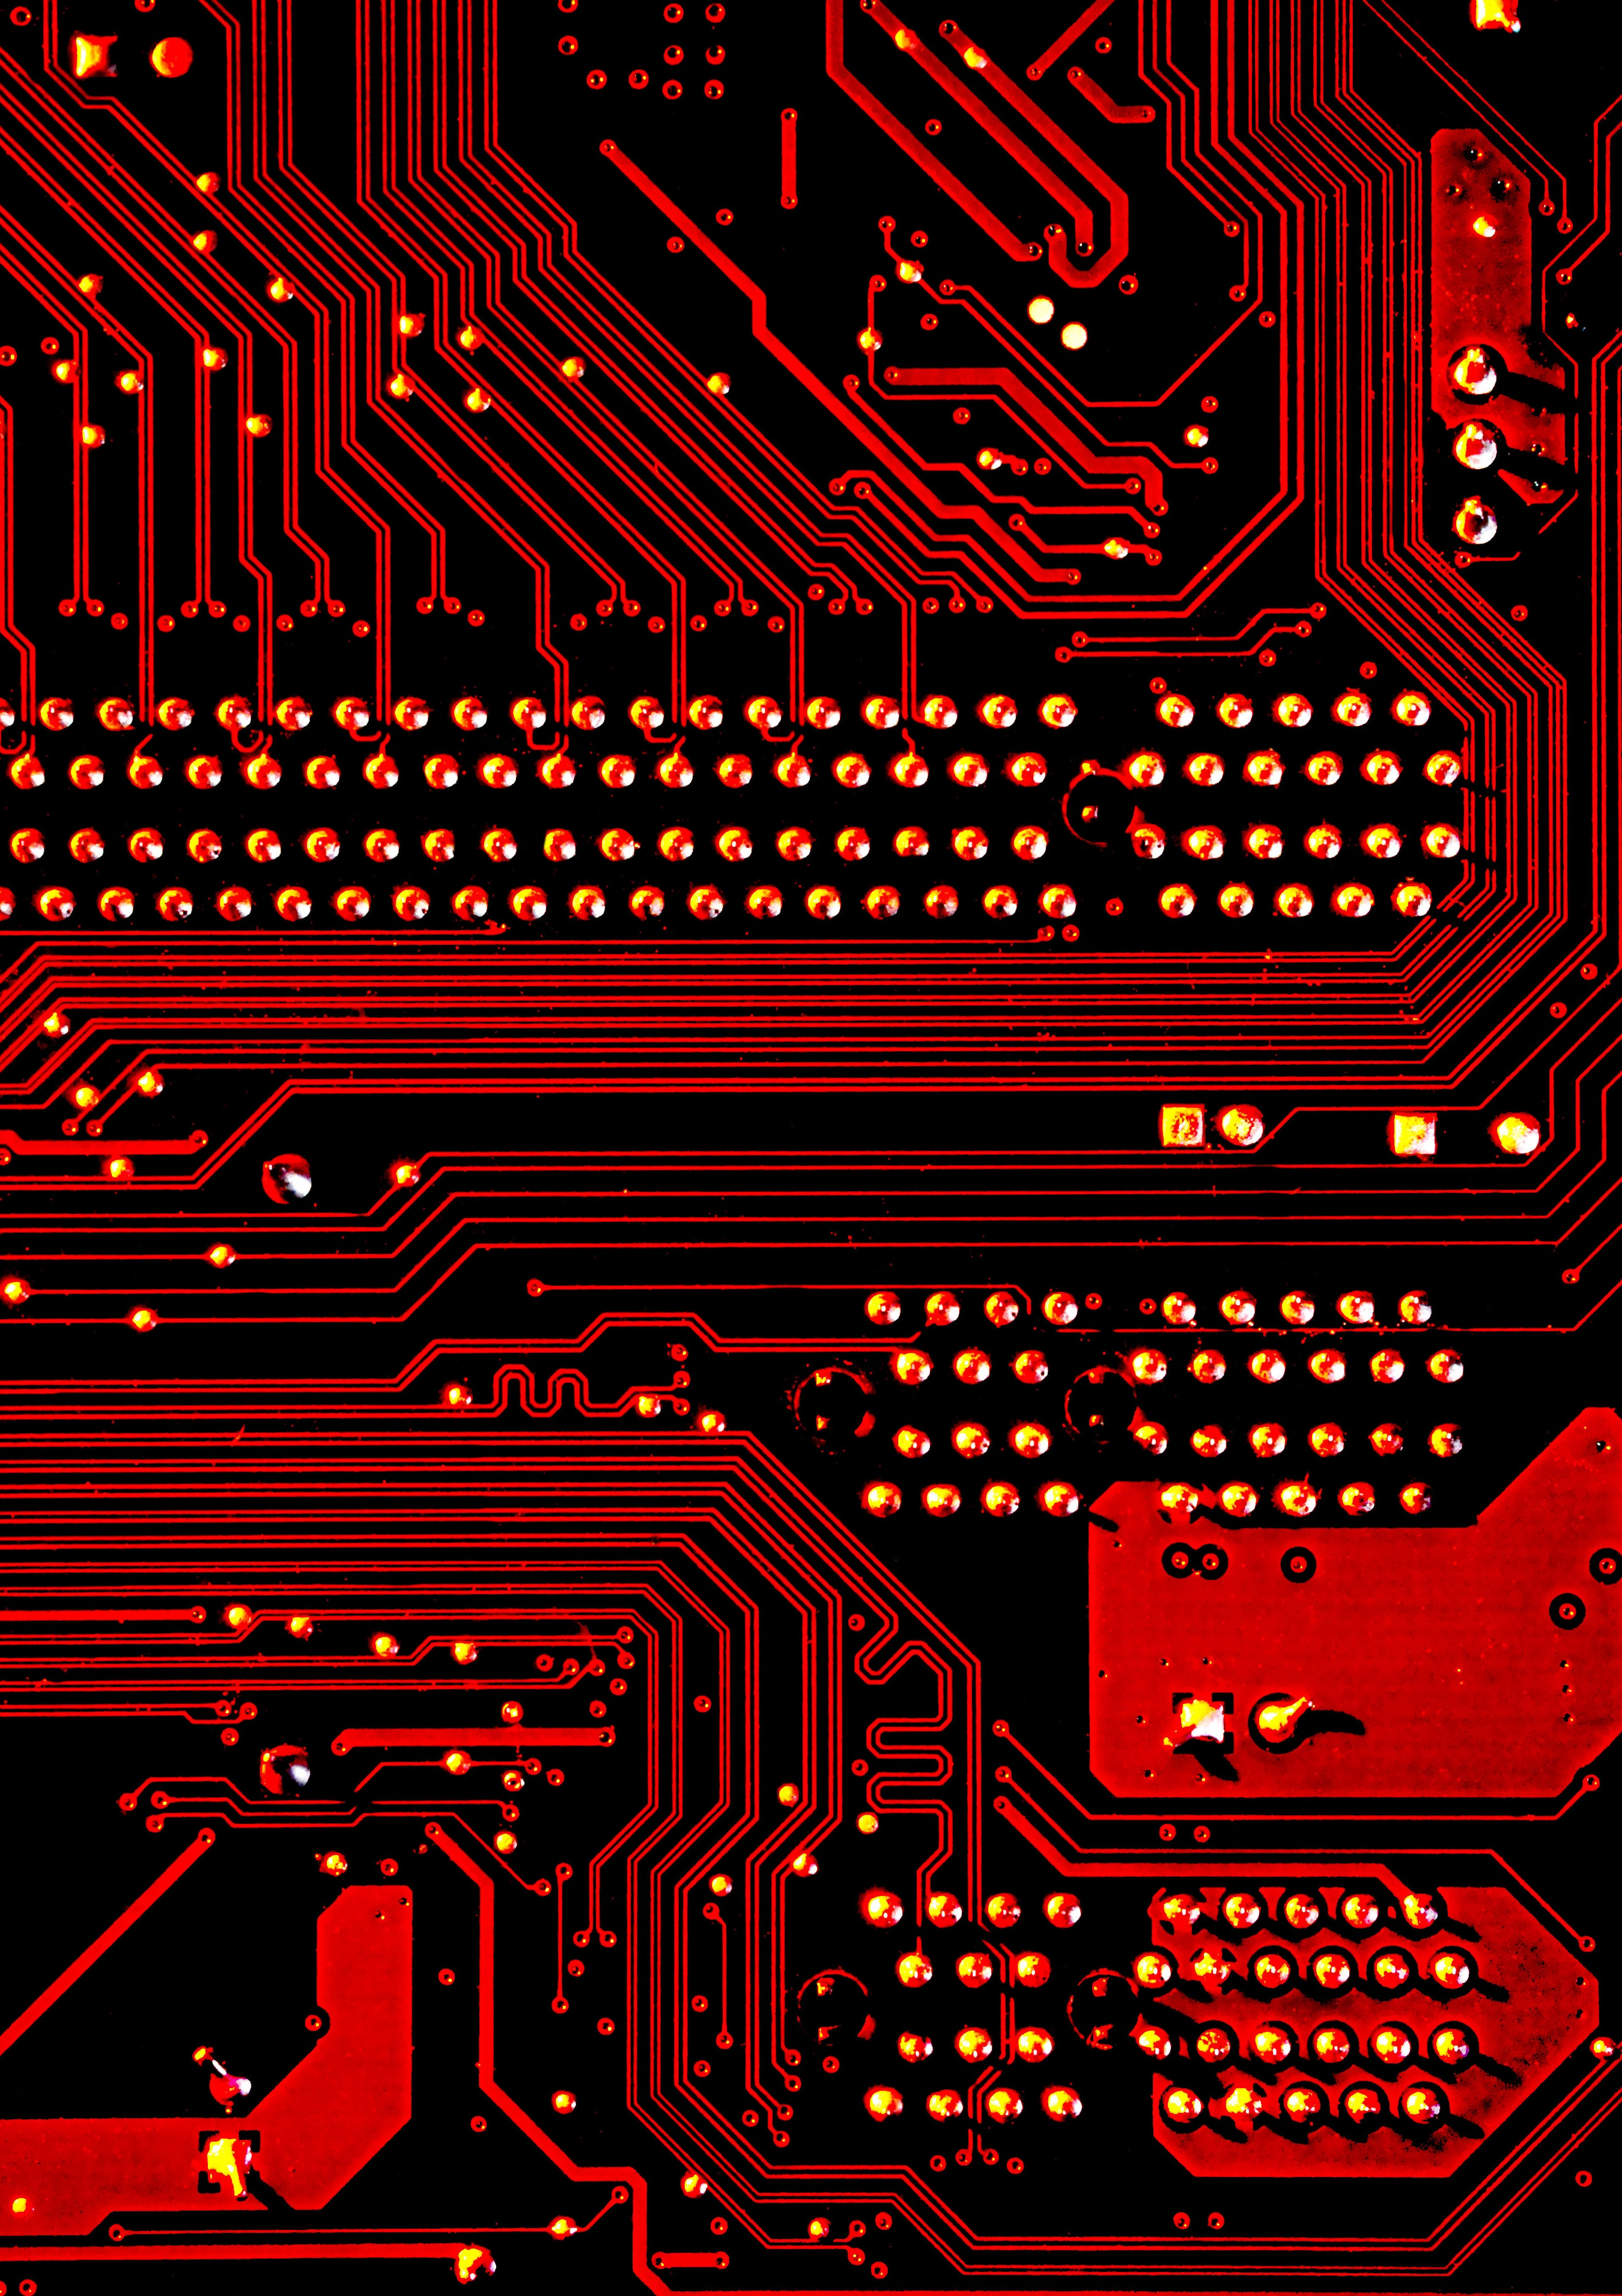
\includegraphics[width=\paperwidth,height=\paperheight]{background.jpg}};

\maketitle
\tcbset{colframe=UCLmidgreen,center title,fonttitle=\bfseries\Large,toptitle=1.5mm,bottomtitle=1.5mm,boxrule=0.8mm,sharp corners,nobeforeafter}
\definecolor{c1}{HTML}{ff7568} 
\definecolor{c2}{HTML}{8cbfff} 
\definecolor{c3}{HTML}{a6ddb7} 
\newcommand{\strutm}{\rule[-.15\baselineskip]{0pt}{\baselineskip}}

\begin{tcolorbox}[title=Introduction]
	\begin{Row}\begin{Cell}{2}
	\textbf{Motivation:}\\
	RISC (Reduced Instruction Set Computer) architecture is usually chosen over CISC (Complex Instruction Set Computer) due to simplicity and lower power consumption. This project goes one step further and investigates OISC (One Instruction Set Computer) MOVE variant architecture to determinate if it can achieve even better performance.
	\end{Cell}\begin{Cell}{2}
	\textbf{About:}\\
	The aim of this project was to design two novel RISC and OSIC architectures with following points:
	\begin{description}
		\item[$\bullet$] Design processors such that could be used for microcontroller application (like 8-bit Atmel AVR)
		\item[$\bullet$] Use same design criteria to make fair comparison
		\item[$\bullet$] Implement processors on FPGA board
		\item[$\bullet$] Design an assembly compiler and common functions
	\end{description} 
	\end{Cell}\begin{Cell}{1}
	\textbf{Decided design criteria:}
	\begin{description}
		\item[$\bullet$] Minimal instruction size
		\item[$\bullet$] Minimalistic design
		\item[$\bullet$] 8bit data bus width
		\item[$\bullet$] 16bit ROM address width
		\item[$\bullet$] 24bit RAM address width
		\item[$\bullet$] 16bit RAM word size
	\end{description}
	\end{Cell}\end{Row}
\end{tcolorbox}

\begin{multicols}{2}

\begin{tcolorbox}[title=RISC Architecture]
	Microarchitecture inspired by MIPS. Separate control and datapath.\\[5mm]
	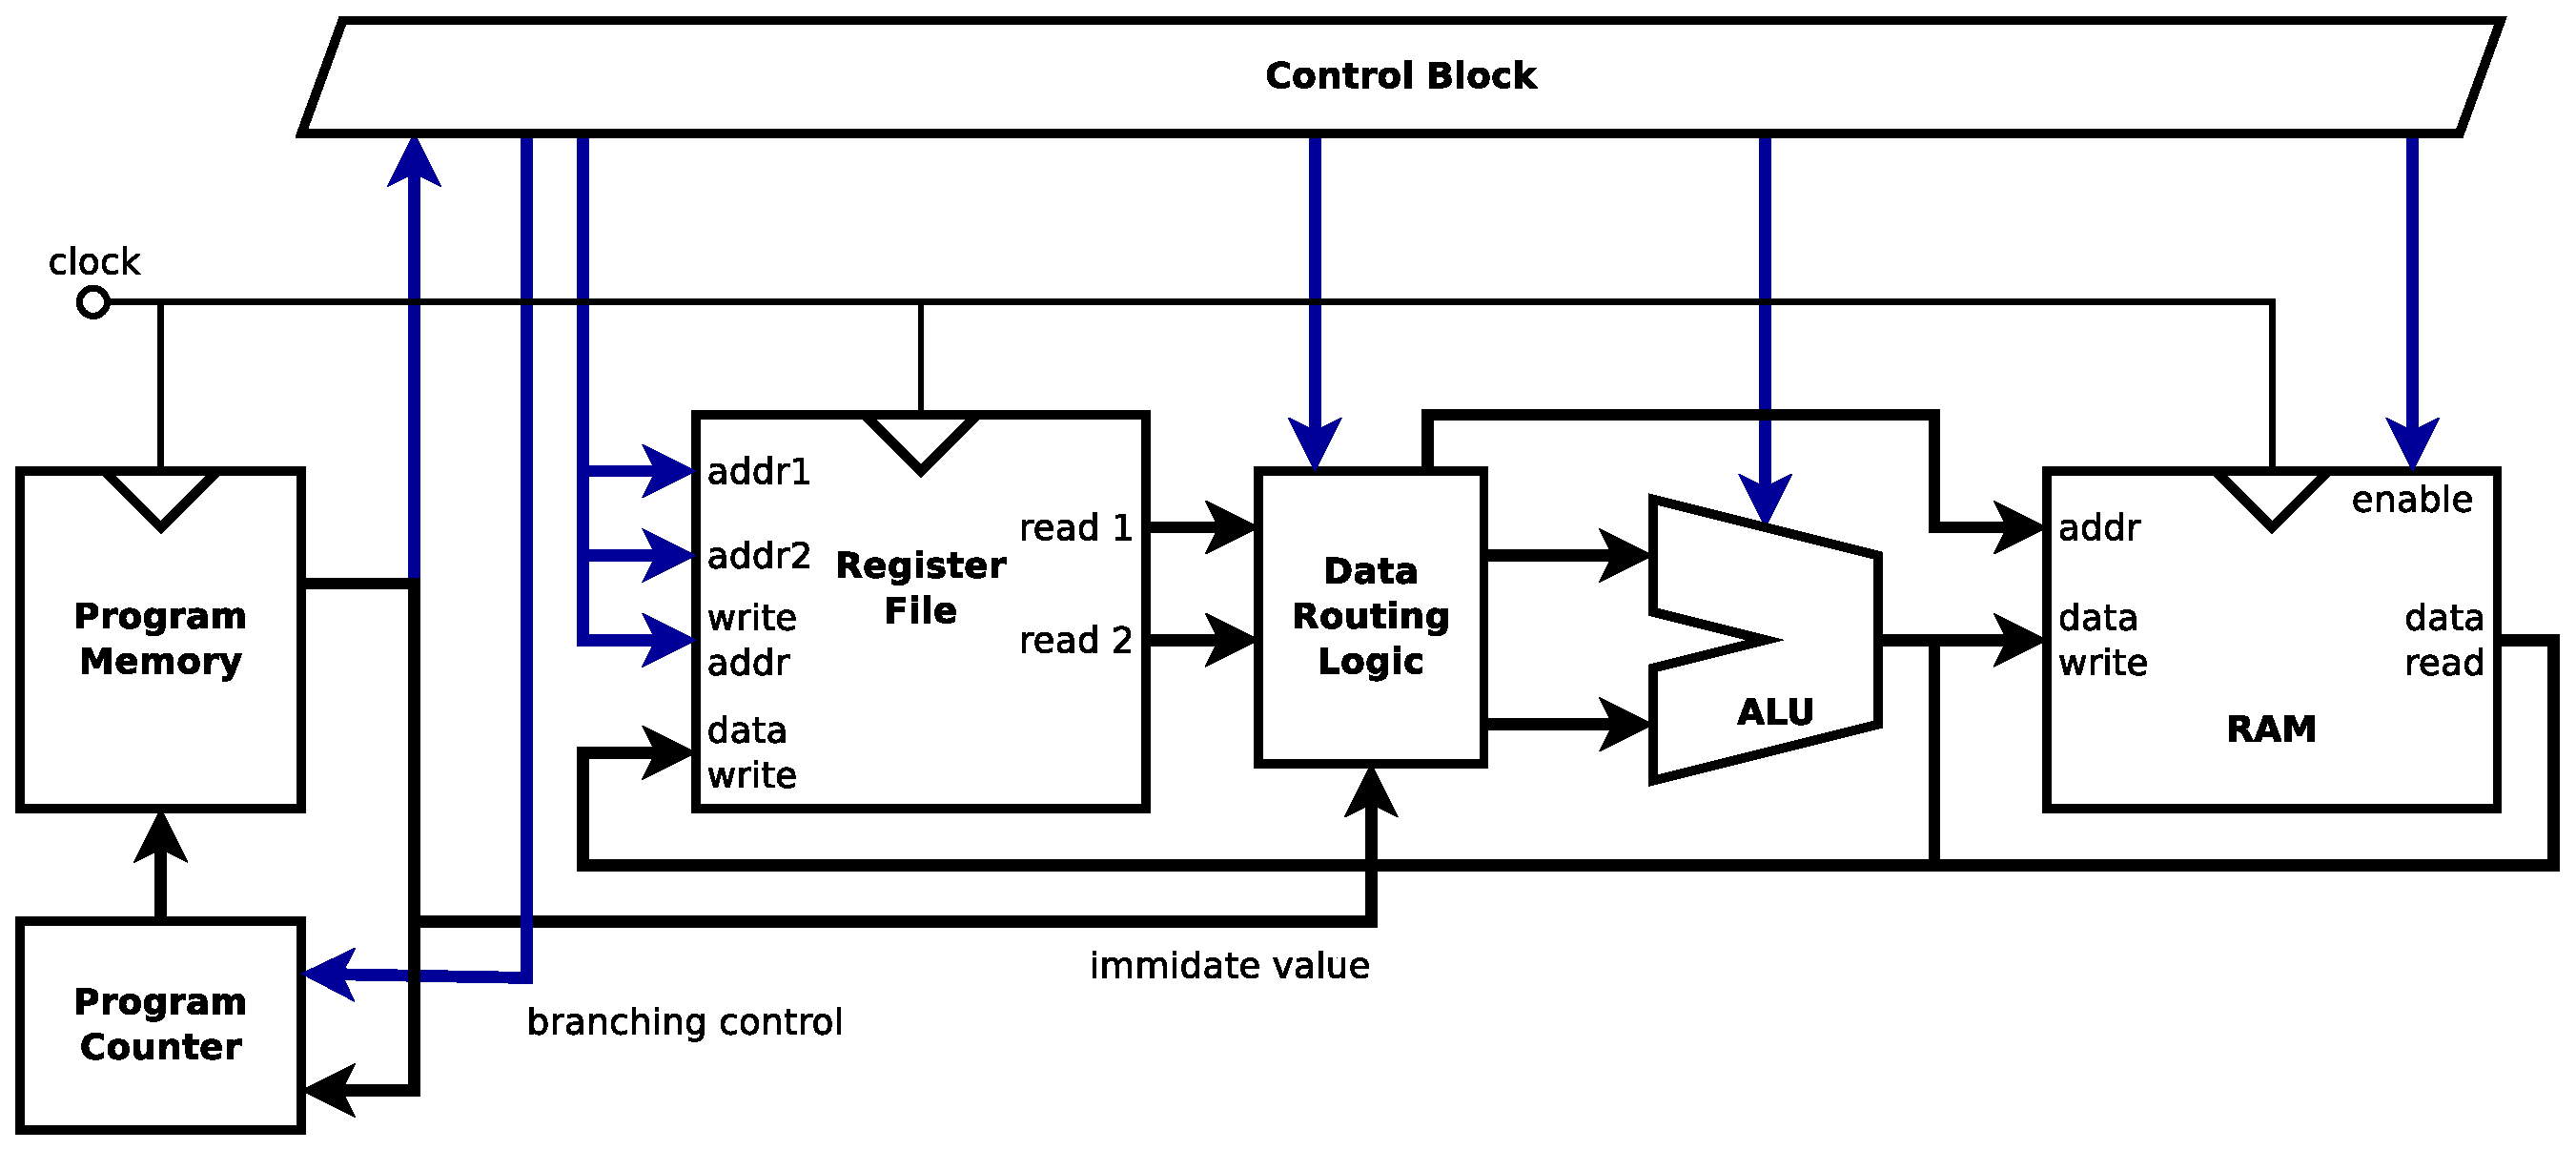
\includegraphics[width=\linewidth]{../resources/risc.eps}
	\begin{center}
	\textit{Figure 1: RISC architecture general block diagram}
	\end{center}
	
\end{tcolorbox}
\begin{tcolorbox}[detach title,beforeafter skip=15pt]
	\textbf{Machine code}\\
	RISC has three types of instructions - with 2, 1 and 0 operands maximising space efficiency. Each type can have from 0 to 3 additional immediate bytes.
	\begin{gather*}
	\scalebox{0.8}{bit index:}
	\overbracket{
		\underbrace{
			\colorbox{c1}{\strutm0}\,
			\colorbox{c1}{\strutm1}\,
			\colorbox{c1}{\strutm2}\,
			\colorbox{c1}{\strutm3}
		}_\text{op. code}
		\underbrace{
			\colorbox{c2}{\strutm4}\,
			\colorbox{c2}{\strutm5}
		}_\text{dst.}
		\underbrace{
			\colorbox{c3}{\strutm6}\,
			\colorbox{c3}{\strutm7}
		}_\text{src.}
	}^\text{2\ operands}
	\quad
	\overbracket{
		\underbrace{
			\colorbox{c1}{\strutm0}\,
			\colorbox{c1}{\strutm1}\,
			\colorbox{c1}{\strutm2}\,
			\colorbox{c1}{\strutm3}
		}_\text{op. code}
		\underbrace{
			\colorbox{c2}{\strutm4}\,
			\colorbox{c2}{\strutm5}
		}_\text{dst.}
		\underbrace{
			\colorbox{c1}{\strutm6}\,
			\colorbox{c1}{\strutm7}
		}_\text{op. c.}
	}^\text{1\ operand}
	\quad
	\overbracket{
		\underbrace{
			\colorbox{c1}{\strutm0}\,
			\colorbox{c1}{\strutm1}\,
			\colorbox{c1}{\strutm2}\,
			\colorbox{c1}{\strutm3}\,
			\colorbox{c1}{\strutm4}\,
			\colorbox{c1}{\strutm5}\,
			\colorbox{c1}{\strutm6}\,
			\colorbox{c1}{\strutm7}
		}_\text{operation code}
	}^\text{0\ operands}
	\end{gather*}
	\\[-13mm]
	\begin{multicols}{2}
	\textbf{45 Total instructions:}
	\begin{description}
		\item[$\bullet$] \textbf{8 }\hspace*{0.5cm} 2-operand instructions
		\item[$\bullet$] \textbf{28}\hspace*{0.5cm} 1-operand instructions
		\item[$\bullet$] \textbf{9 }\hspace*{0.5cm} 0-operand instructions
	\end{description}
	\columnbreak
	\begin{description}
		\item[$\bullet$] \textbf{4}\hspace*{0.2cm} General purpose registers
		\item[$\bullet$] Hardware stack
		\item[$\bullet$] Hardware multiply / divide
		\item[$\bullet$] Hardware call / return
	\end{description}
	\end{multicols}

\end{tcolorbox}

\columnbreak

\begin{tcolorbox}[title=OISC Architecture]
	Common data and instruction bus. No control block. Data is moved around using single MOVE instruction by enabling buffers connected to data bus.\\[5mm]
	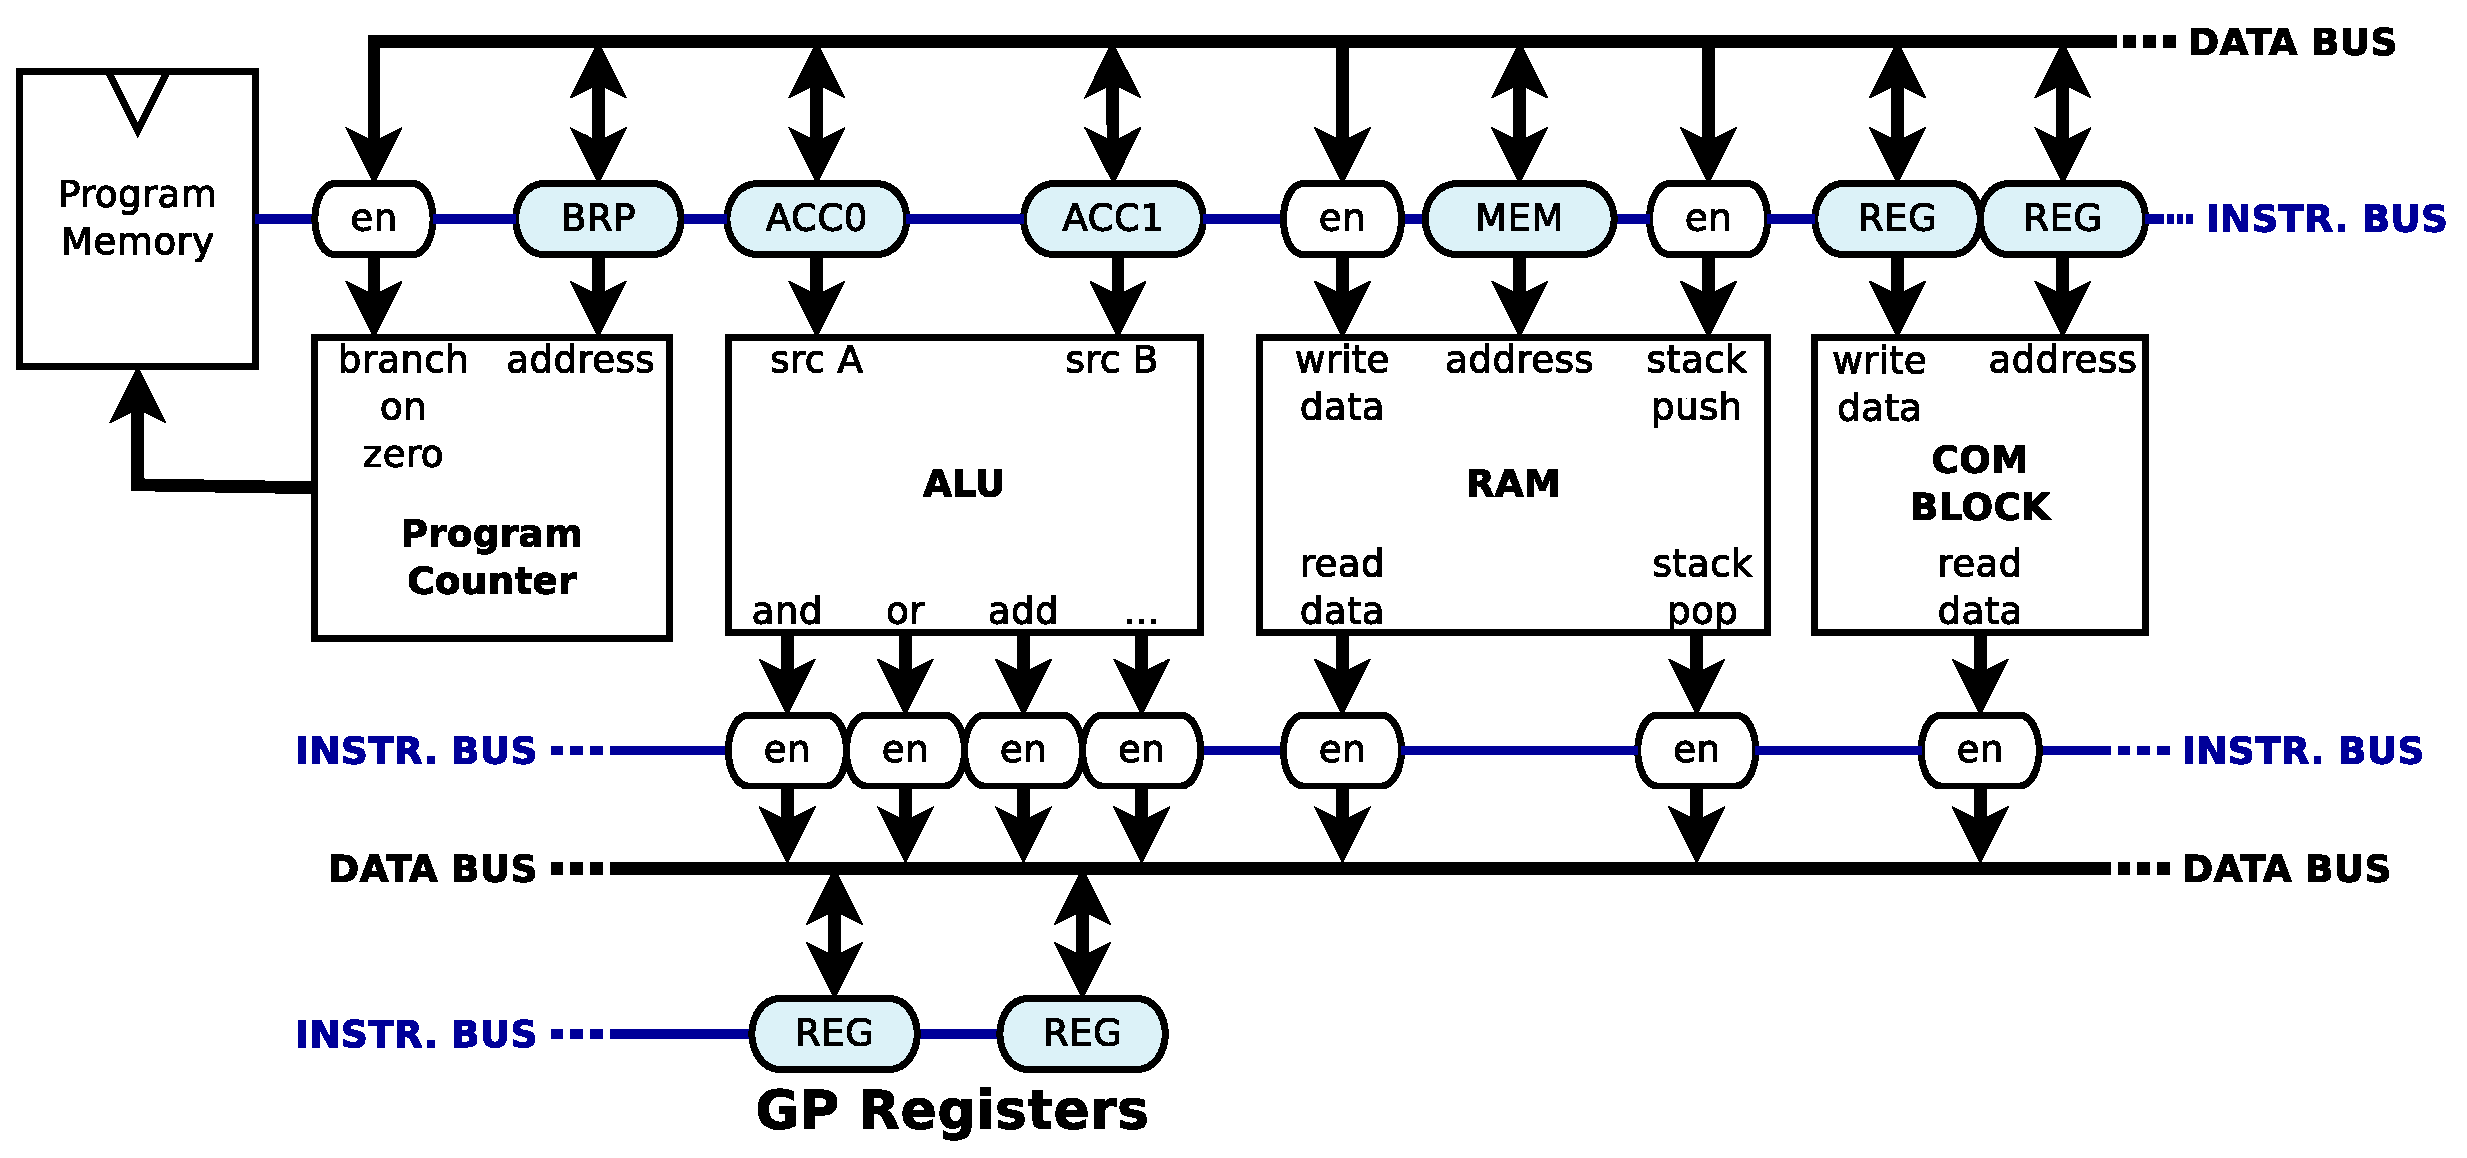
\includegraphics[width=\linewidth]{../resources/oisc.eps}
	\begin{center}
	\textit{Figure 2: OISC architecture general block diagram}
	\end{center}
\end{tcolorbox}
\begin{tcolorbox}[detach title,beforeafter skip=26pt]
	\textbf{Machine code}\\
	OISC instructions are fixed 13bit width, 1 bit to set source as immediate value, 4bits for destination address and 8bit for source or immediate.
	\\
	\begin{gather*}
	\scalebox{0.8}{bit index:}
	\underbrace{
		\colorbox{c1}{\strutm0}
	}_\text{imm.}
	\underbrace{
		\colorbox{c2}{\strutm1}\,
		\colorbox{c2}{\strutm2}\,
		\colorbox{c2}{\strutm3}\,
		\colorbox{c2}{\strutm4}\,
	}_\text{destination}
	\underbrace{
		\colorbox{c3}{\strutm5}\,
		\colorbox{c3}{\strutm6}\,
		\colorbox{c3}{\strutm7}\,
		\colorbox{c3}{\strutm8}\,
		\colorbox{c3}{\strutm9}\,
		\colorbox{c3}{\strutm10}\,
		\colorbox{c3}{\strutm11}\,
		\colorbox{c3}{\strutm12}
	}_\text{source}
	\end{gather*} 
	\\[-13mm]
	\begin{multicols}{2}
	\begin{description}
		\item[$\bullet$] \textbf{15}\hspace*{0.2cm} Destination addresses
		\item[$\bullet$] \textbf{41}\hspace*{0.2cm} Source addresses
		\item[$\bullet$] \textbf{2}\hspace*{0.2cm} General purpose registers
		\columnbreak
		\item[$\bullet$] Hardware stack
		\item[$\bullet$] Hardware multiply / divide
		\item[$\bullet$] Software call / return
	\end{description}
	\end{multicols}
\end{tcolorbox}

\end{multicols}


\begin{tcolorbox}[title=Results]
	\begin{multicols}{3}
		\textbf{Implemented functions in assembly:}
		\begin{description}
			\item[$\bullet$] Print Strings, values in Binary, Hexadecimal and Decimal (8 and 16bit)
			\item[$\bullet$] 16bit multiplication
			\item[$\bullet$] 16bit division
			\item[$\bullet$] 16bit modulus
			\item[$\bullet$] Sieve of Atkins (prime number calculator, up to 16bit number)
		\end{description}
		\vfill
		\begin{center}
			\renewcommand{\arraystretch}{1.5}
			\begin{tabular}{ | l | c | c | c | }
				\hline
				& \textbf{Baseline} & \textbf{RISC} & \textbf{OISC} \\ \hline
				Logic Elements 	& 293 & 1771 & 1705 \\ \hline
				Registers 		& 169 & 602 & 724  \\ \hline
			\end{tabular}
		\\[2mm]
		\textit{Table 1: Number of FPGA resources}
		\end{center}

		\columnbreak
		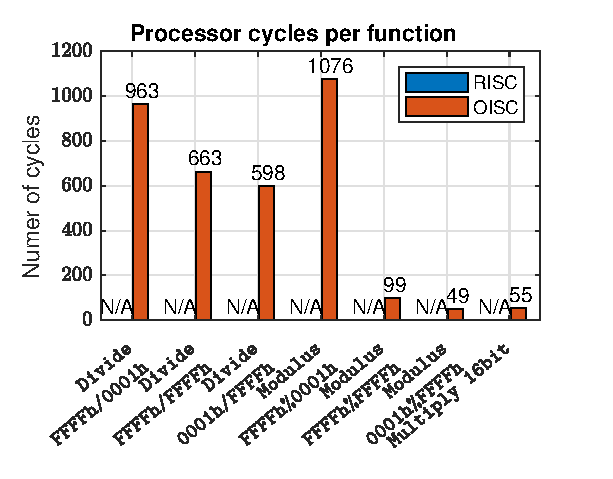
\includegraphics[width=\linewidth]{../tests/cycles.eps}
		\begin{center}
			\textit{Figure 3: Simulated results of cycles that taken to perform function. }
		\end{center}
	
		\columnbreak
		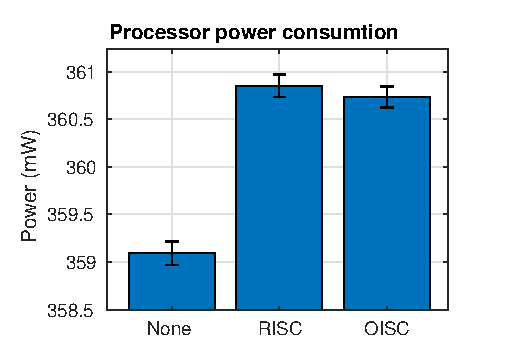
\includegraphics[width=\linewidth]{../tests/power.eps}
		\begin{center}
			\textit{Figure 4: Measured power of processors when implemented on FPGA, running 16bit multiplication function in loop.}
		\end{center}

	\end{multicols}
	
%	\renewcommand{\arraystretch}{1.5}
%	\begin{Row}\begin{Cell}{2}
%		\textbf{Implemented functions in assembly:}
%		\begin{description}
%			\item[$\bullet$] Print ASCII, Binary, Hexadecimal and Decimal (8 and 16bit)
%			\item[$\bullet$] 16bit multiplication
%			\item[$\bullet$] 16bit division - 
%			\item[$\bullet$] 16bit modulus
%			\item[$\bullet$] Sieve of Atkins (prime number calculator)
%		\end{description}
%	\end{Cell}\begin{Cell}{2}
%		\textbf{Number of cycles per function:}
%		\begin{center}
%		\begin{tabular}{ | l | c | c | }
%			\hline
%			\textbf{Function} & \textbf{RISC} & \textbf{OISC} \\ \hline
%			16bit division \texttt{FFFFh/0001h} & - & 963 \\ \hline
%			16bit division \texttt{FFFFh/FFFFh} & - & 663 \\ \hline
%			16bit division \texttt{0001h/FFFFh} & - & 598 \\ \hline
%			16bit modulus \texttt{FFFFh\%0001h} & - & 1076 \\ \hline
%			16bit modulus \texttt{FFFFh\%FFFFh} & - & 99 \\ \hline
%			16bit modulus \texttt{0001h\%FFFFh} & - & 49 \\ \hline
%			16bit multiply & - & 55  \\ \hline
%		\end{tabular}
%		\end{center}
%	
%		\textbf{Number of FPGA resources:}
%		\begin{center}
%		\begin{tabular}{ | l | c | c | c | }
%			\hline
%			& \textbf{Baseline} & \textbf{RISC} & \textbf{OISC} \\ \hline
%			Logic Elements 	& 293 & 1771 & 1705 \\ \hline
%			Registers 		& 169 & 602 & 724  \\ \hline
%		\end{tabular}
%		\end{center}
%		\textbf{Power consumption (mW):}
%		\begin{center}
%		\begin{tabular}{ | c | c | c | }
%			\hline
%			\textbf{Baseline} & \textbf{RISC} & \textbf{OISC} \\ \hline
%			359.09 $\pm$ 0.245 & 360.851 $\pm$ 0.239 & 360.732 $\pm$ 0.223 \\ \hline
%		\end{tabular}
%		\end{center}
%	\end{Cell}\begin{Cell}{2}
%		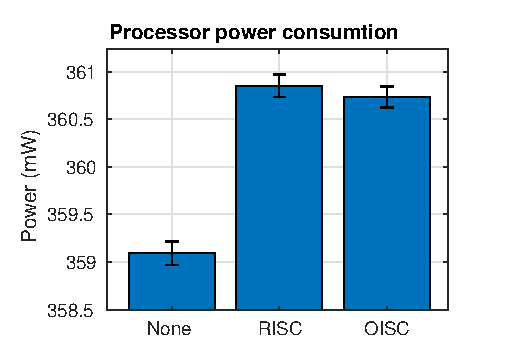
\includegraphics[width=\linewidth]{../tests/power.eps}
%	
%	\end{Cell}\end{Row}
\end{tcolorbox}

\begin{Row}\begin{Cell}{1}

\begin{tcolorbox}[title=Conclusion]
	\begin{description}
		\item[$\bullet$] Processor achieved similar performance in power consumption and FPGA resources
		\item[$\bullet$] OISC seems to be \textbf{easier} to implement and expand, easily enabling \textbf{pipelining} with hazard control implemented by software.
		\item[$\bullet$] OISC takes more instructions to perform same function.
		\item[$\bullet$] OISC assembly is more difficult to write.
		\item[$\bullet$] Further research is need to investigate benefits of multi-data-bus OISC design.
		\\[1mm]
	\end{description}
\end{tcolorbox}	

\end{Cell}\begin{Cell}{2}

\begin{tcolorbox}[title=Future work]
	\begin{multicols}{2}
		\textbf{Write more tests:}
		\begin{description}
			\item[\textendash] Test Spongent (crypto-hashing) algorithm
			\item[\textendash] Array and matrix calculations (sorting, search, calculating mean, etc.)
			\item[\textendash] Other minimalistic cryptographic functions
		\end{description}
	
		\textbf{Short term work:}
		\begin{enumerate}
			\item Investigate critical path and maximum frequencies
			\item Find power activity factor
			\item Implement OISC emulator for easier debugging
		\end{enumerate}
		\columnbreak
		\textbf{Future research:}
		\begin{enumerate}
			\item Implement multiple data \& instruction buses for OISC
			\item Write higher level language compiler (such as BASIC or C)
			\item Expand to 16bit / 32bit data bus
			\item Compare to commercial Atmel AVR / ARM / MIPS  architectures
		\end{enumerate}
	\end{multicols}

\end{tcolorbox}
\end{Cell}\end{Row}

\end{document}
